% samplepaper.tex: springer.com
% modificato da MM 06/05/2018
%
\documentclass[runningheads]{llncs}


\usepackage[a4paper, total={6in, 9in}]{geometry}


\usepackage[italian]{babel}
\usepackage{graphicx}
\usepackage{listings}
\usepackage{threeparttable}
\usepackage{tipa}
\usepackage{tikz}
\usepackage{subfig}
\usepackage{graphicx} % for "\includegraphics" macro
% Used for displaying a sample figure. If possible, figure files
% should be included in EPS format.  If you use the hyperref package,
% please uncomment the following line to display URLs in blue roman
% font according to Springer's eBook style:
% \renewcommand\UrlFont{\color{blue}\rmfamily}
\begin{document}
%
\title{Classificazione articoli ANSA via topic modelling}
%
% \titlerunning{Abbreviated paper title}
% If the paper title is too long for the running head, you can set
% an abbreviated paper title here
%
\author{%
  Alessandro Stefani\inst{1} e
  Cristi Gutu\inst{2}}
%
\authorrunning{Alessandro Stefani, Cristi Gutu}
% First names are abbreviated in the running head.  If there are more
% than two authors, 'et al.' is used.
%
\institute{Corso di laurea in Statistica per le tecnologie e le scienze, nome d'arte Aleste
%\footnote{famoso persuasore sulla piattaforma Tinder, swipe right @asteph7cd}
  matricola 1148387 \email{alessandro.stefani.6@studenti.unipd.it} \and Corso di laurea in Statistica per le tecnologie e le scienze,
      matricola 1147351 \email{gheorghecristi.gutu@studenti.unipd.it}
  }
%
\maketitle
% typeset the header of the contribution
%
\begin{abstract}
Questo progetto tratta la realizzazione di un classificatore di notizie in macro categorie provenienti dall'agenzia ANSA. 
Come scopo primario e' stato fissato la massimizzazione dell'accuratezza del classificatore, cioe' il valore definito dall'espressione = ($\frac{ Previsioni\_corrette}{Totale\_tentativi\_previsione}$), in quanto, avendo un numero di osservazioni bilanciato per classe e con classi di equa importanza, non si rischia di incorrere nel paradosso dell'accuratezza. Sono state sfruttate tecniche di analisi dei testi,  tra cui: Latent Dirchlet Allocation\cite{LDA},
Alberi di decisione\cite{tree}, raggruppamento  in n-grammi\cite{NGRAM} dei termini.
 \keywords{{\it
      Classification  \and Text mining  \and Text classification \and n-gram \and LDA \and Python \and sklearn}}
\end{abstract}

\section{Introduzione}
\label{sec:introduzione}
In questo progetto vogliamo confrontare l'efficacia di alcuni modelli di rappresentazione dei documenti nel problema di classificazione, in particolare ci concentriamo su: LDA, Term Frequency e Term Frequency basato su n-grammi. 



%
%\section{Metodi proposti}
%\label{sec:metodi-utilizzati}
%
%Nel caso in cui si siano sviluppati:
%\begin{itemize}
%\item modelli di reperimento,
%\item metodi di indicizzazione,
%\item schemi di pesatura o
%\item altri metodi o tecniche
%\end{itemize}
%propri, non documentati in libri di testo o altra letteratura, si
%scriva in questa sezione una descrizione accurata e completa.  Si
%mettano in evidenza le caratteristiche distintive dei propri
%contributi.  Se non si \`e proposto nulla di nuovo, si scriva
%\emph{Nessuno}.  In una delle ultime lezioni si vedr\`a come
%implementare delle proprie funzioni di reperimento e schemi di
%pesatura.

\section{Dataset}
\label{sec:dataset}

I dati sono stati reperiti dall'agenzia ANSA, nota in Italia. Il campionamento degli articoli e' stato fatto ottenendo i link traminte il motore di 
ricerca DuckDuckGo. Si e' deciso di includere 6 macro categorie: (Economia, Politica, Cultura, Sport, Tecnologia, Cronaca), escludendo la categoria Mondo perche' si confonde con categorie come Economia e Politica, per
ogni categoria sono stati reperiti 400 articoli sfruttando la ricerca mirata solo al sito ansa.it via le espressioni:
\begin{itemize}
\item site:ansa.it/sito/notizie/economia
\item site:ansa.it/sito/notizie/politica
\item site:ansa.it/sito/notizie/cultura
\item site:ansa.it/sito/notizie/sport
\item site:ansa.it/sito/notizie/tecnologia
\item site:ansa.it/sito/notizie/cronaca
\end{itemize}

Cercando con queste espressioni si reperiscono risultati che appartengono soltanto ai temi citati sopra.

Ogni articolo e' composto da: (titolo, sottotitolo, testo, tags, categoria). Le tags sono parole chiavi che dovrebbero aiutare il 
lettore a contestualizzare il contenuto dell'articolo e di conseguenza categorizzarlo in qualche maniera.
Si sono estratte da ogni articolo i campi citati sopra i cui valori sono stati salvati in formato JSON\footnote{formato di serializzazione per dati}. 

In totale si sono raccolti 2400 articoli\footnote{Dataset scaricabili in formato json all'inidirizzo:
 \url{$https://github.com/mastershef/big\_data}$}, che sono stati suddivisi casualmente in training set,
validation set e test set.





\section{Esperimenti}
\label{sec:esperimenti}

% esperimento 1: cambio numero componenti LDA e accuratezza
% esperimento 2: accuratezza cambiando numerosita insieme training con LDA
% esperimento 3: accuratezza cambiando numerosita insieme training senza LDA
% esperimento 4: accuratezza cambiando numerosita insieme training senza LDA




Prima di poter utilizzare modelli per l'analisi testuale è necessario preprocessare i dati,
questo e' stato fatto costruendo la seguente pipeline di preprocessamento: articoli \textpipe  rimozione stopwords\footnote{Utilizzando le parole dalla libreria TextWiller github.com/livioivil/TextWiller} \textpipe  stemming \textpipe rimozione tags html \textpipe rimozione punteggiatura \textpipe rimozione numeri \textpipe rimozione link.


\subsection{Baseline}
\label{sec:baseline}

Come basline si e' deicso di classificare utilizzando il modello $\it DummyClassifier$ che classifica ogni articolo secondo la categoria piu' frequente del training set. L'accuratezza ottenuta e' del: 15\%.


\subsection{Analisi esplortive}
Si e' notato che le categorie assegnate agli articoli erano in realta' micro-cateogire, percio' un ultimo step 
di preprocessamento e' stato riclassificare manualmente gli articoli, etichettandoli con le corrispondenti macro-categorie.

Ad esempio: Cultura $\leftarrow $ (Libri, Cinema, Film); gli articoli con micro-categoria Libri o Cinema o Film, vengono rietichettati con la macro-categoria Cultura.

Successivamente si e' calcolata la term-document matrix\footnote{e' una matrice che ha sulle colonne le singole parole e sulle righe 0 o 1 che indicano se la parola e' presente nel documento alla riga i oppure no e se' presente piu' volte nella cella e' memorizzato il numero di volte che compare in quel documento, calcolato attraverso    $sklearn.feature\_extraction.text.CountVectorizer$}  la cui classe di supporto in Python da' la possibilita' di specificare 3 parametri: ngram\_range, min\_df, max\_df; per scegliere il
range di ngrammi da prendere in considerazione si e' fatto riferimento al libro Social Media e Sentiment Analysis\cite{NGRAM} dove si suggerisce che generalmente n-grammi con piu' di 3 termini non aggiungono contenuto informativo, i parametri max\_df, min\_df sono invece stati scelti in base alla distribuzione delle "frequenze degli ngrammi nei documenti" del train set.


Per continuare l'esplorazione, si e' cercato di visualizzare come i dati sono raggrupati in categorie riducendo lo spazio delle features con tSNE, l'approccio iniziale e' consistito nell'utilizzare la term document matrix
come insieme di variabili esplicative, seguendo la pipeline: articoli preprocessati \textpipe Term Document Matrix \textpipe tSNE a 3 componenti.

\begin{figure}%
    \centering
    \subfloat[Vista normale]{{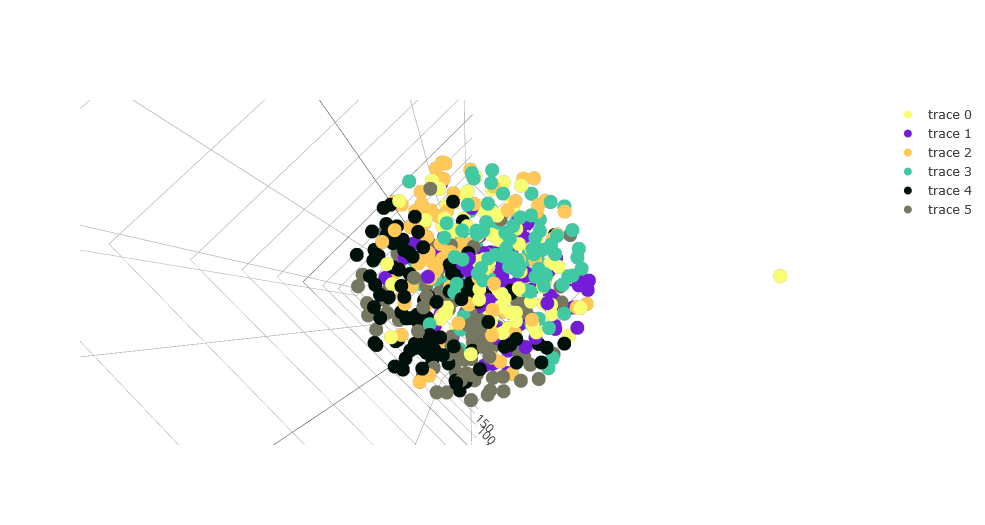
\includegraphics[width=.45\linewidth]{tsne-1-1} }}%
    \qquad
    \subfloat[Vista ravvicinata]{{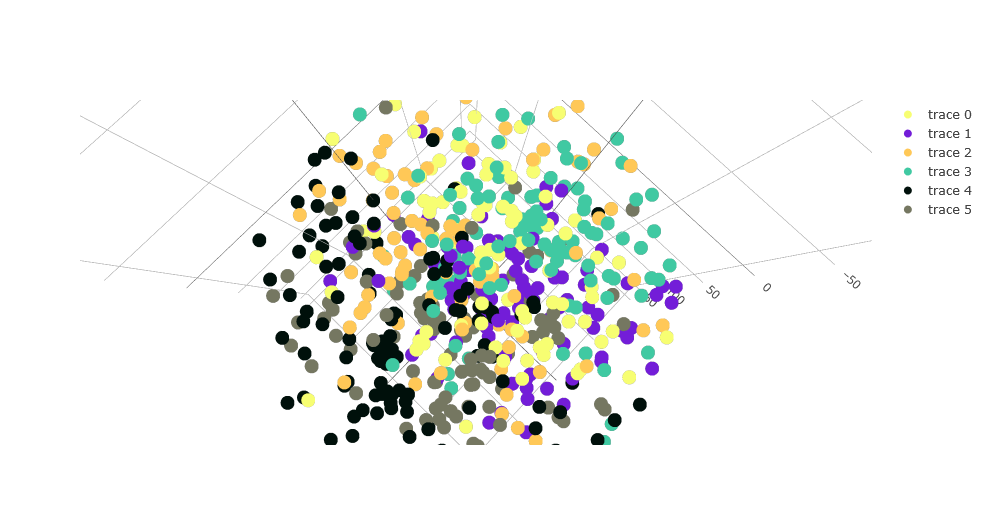
\includegraphics[width=.45\linewidth]{tsne-1-2} }}%
    \caption{Riduzione della term document matrix da forma (2400, 4640) a forma (2400, 3) via tSNE. }%
    \label{fig:tsne1}%
\end{figure} 

Si vede in Figura 1 come articoli dello stesso tema sono abbastanza distaziati tra loro e sparsi nell'agglomerato di 
articoli.\par

\qquad
\qquad



Successivamente si e' provato attraverso la stessa pipeline, applicando in piu' Latent Dirichlet Allocation (LDA), impostando come parametri n\_components \footnote{numero di topic latenti che LDA dovrebbe individuare} a 6 e learning\_decay\footnote{parametro usato per regolare il \"learning rate\", che si consiglia imposare nel range (0.5, 1] per garantire la convergenza asintotica.} al valore di default.



%quelli della classe CountVectorizer: ngram\_range\footnote{ampiezza intervallo degli n-grammi da considerare}, min\_df\footnote{minimo document frequency, cioe' il minimo numero di volte che una parola deve apparire in un documento affinche' questa venga inclusa nel vettore di conteggio.}, max\_df\footnote{controparte di min\_df}; e quelli del classificatore via Alberi: min\_samples\_leaf\footnote{indica il numero di osservazioni minimo per ogni foglia}, max\_depth\footnote{indica la profondita' massima dell'albero}.




\begin{figure}%
    \centering
    \subfloat[Vista normale]{{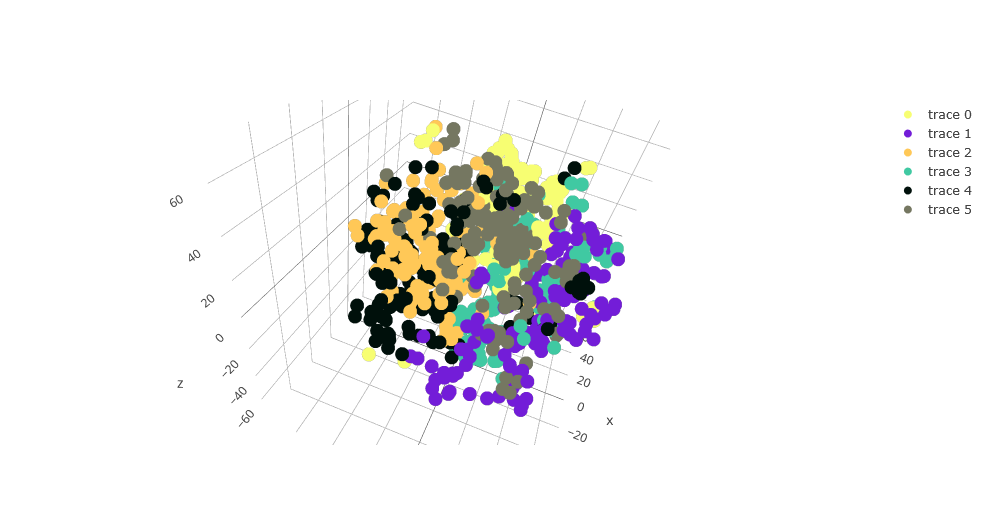
\includegraphics[width=.45\linewidth]{tsne_ottimizzato-1} }}%
    \qquad
    \subfloat[Vista ravvicinata]{{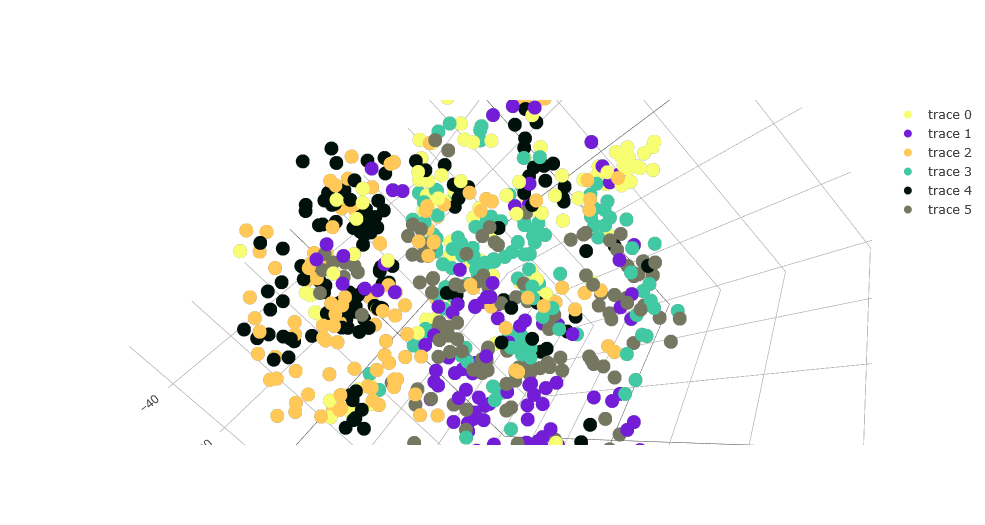
\includegraphics[width=.45\linewidth]{tsne_ottimizzato} }}%
    \caption{Riduzione della matrice da forma (2400, 4640) a forma (2400, 3). }%
    \label{fig:tsne2}%
\end{figure}


A differenza della Figura 1 in questa figura (esplorazione interattiva
\footnote{https://plot.ly/create/?fid=cristi.gutzu:5\&fid=cristi.gutzu:6}) si vede come i diversi temi sono raggruppati in piccoli cluster sparsi in maniera piu' o meno uniforme lungo i tre assi, inoltre articoli dello stesso tema nella Figura 2 sembrano essere meno distanti tra loro. Sempre dalla Figura 2 si evince come un albero potrebbe essere una soluzione accettabile per il problema di classificazione.

\subsection{Prove}

Si e' deciso di mettere a confronto 3 configurazioni attraverso le quali si vede come l'accuratezza delle predizioni
varia al variare della dimensione del training set. Nella seguente tabella si evincono le 3 configurazioni.

\def\checkmark{\tikz\fill[scale=0.3](0,.3) -- (.25,0) -- (1,.7) -- (.25,.15) -- cycle;} 
\begin{table}[]
\centering
\begin{tabular}{llll}
\hline
\textbf{Pipeline} \textbackslash \textbf{Trasformation} & LDA-12 & LDA-48 & Term Frequency \\ \hline
T.D Matrix                  &    \checkmark    & \checkmark      & \checkmark    \\ 
LDA                       & \checkmark      & \checkmark      & x   \\ 
Classifier                & \checkmark      & \checkmark      & \checkmark     \\ \hline
\end{tabular}
\begin{tablenotes}
      \small
      \item  \textbf{Tabella:} configurazioni LDA-12 e LDA-48, indicano i modelli fittati con 12 e 48 componenti.
    \end{tablenotes}
\end{table}


\begin{figure}%
    \centering
    \subfloat{{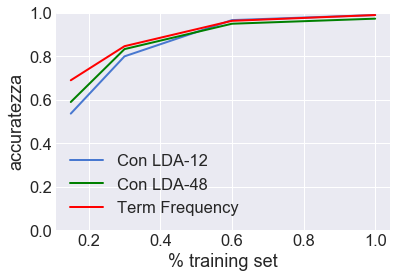
\includegraphics[width=.3\linewidth]{accuracy} }}%
    \caption{Performace modelli di classificazione sul test set in funzione della dimensione del training set.}%
\end{figure} 


\section{Risultati finali}





Come riportato in Tabella 1, le rappresentazioni LDA-12 e Term Frequency hanno pari accuratezza, e sono i modelli migliori tra quelli che abbiamo stimato, classificando gli articoli dell'insieme di test.
\begin{table}[]
    \centering
\begin{tabular}{ll}
\hline
Rappresentazione & Accuratezza      \\ \hline
Dummy            & 15.0 \%          \\
LDA-12           & \textbf{99.0 \%} \\
LDA-48           & 97.3 \%          \\
Term Frequency   & \textbf{99.0 \%} \\ \hline
\end{tabular}
    \caption{Risultati utilizzando i diversi modelli di raprresentazione con l'intero training set.}%
\end{table}
Siccome l'accuratezza, che misura la qualita' complessiva del modello, risulta molto buona, ci si e' chiesto come il classificatore si comporta anche per le singole classi, per verificarlo abbiamo calcolato ulteriori misure per i due modelli migliori.


%
%    'lda__n_components': 12,
%    'lda__learning_decay': 0.7, 
%    'count_mx__ngram_range': (1, 3), 
%    'count_mx__min_df': 10, 
%    'count_mx__max_df': 0.5, 
%    'classifier__min_samples_leaf': 1, 
%    'classifier__max_depth': 22




\begin{table}[]
\centering
\begin{tabular}{lllll}
\hline
Categoria    & precision & recall & f1   & support \\ \hline
Cronaca     & 0.96   &   1.00    &  0.98  & 45      \\
Cultura      & 1.00      & 1.00   & 1.00 & 57      \\
Economia     & 1.00      & 0.98   & 0.99 & 44      \\
Politica     & 1.00      & 0.96   & 0.98 & 54      \\
Sport        & 1.00      & 1.00   & 1.00 & 49      \\
Tech         & 0.98      & 1.00   & 0.99 & 51      \\ \hline
micro avg    & 0.99      & 0.99   & 0.99 & 300     \\ \hline
macro avg    & 0.99      & 0.99   & 0.99 & 300     \\ \hline
weighted avg & 0.99      & 0.99   & 0.99 & 300    \\  \hline
\end{tabular}
    \caption{Report metriche sul classificatore stimato con LDA-12.}%

\end{table}



\begin{table}[]
\centering
\begin{tabular}{lllll}
\hline
Categoria    & precision & recall & f1   & support \\ \hline
Cronaca     & 1.00   &   1.00    &  1.00 & 45      \\
Cultura      & 1.00      & 1.00   & 1.00 & 57      \\
Economia     & 0.96      & 0.98   & 0.97 & 44      \\
Politica     & 1.00      & 0.96   & 0.98 & 54      \\
Sport        & 1.00      & 1.00   & 1.00 & 49      \\
Tech         & 0.98      & 1.00   & 0.99 & 51      \\ \hline
micro avg    & 0.99      & 0.99   & 0.99 & 300     \\ \hline
macro avg    & 0.99      & 0.99   & 0.99 & 300     \\ \hline
weighted avg & 0.99      & 0.99   & 0.99 & 300    \\  \hline
\end{tabular}
    \caption{Report metriche sul classificatore stimato con Term Frequency.}%

\end{table}


Si osserva dalle tabelle che le metriche: precisione, richiamo, f1; sono molto alte per ogni classe, cosa che conferma l'accuratezza elevata ottenuta sul trainig set.


\section{Conclusioni}

Dai risultati delle analisi si vede che il modello basato sulla rappresentazione con LDA e' comparabile al modello basato sulla rappresentazione con Term Frequency dal punto di vista dell'accuratezza, tuttavia il modello con LDA riduce lo spazio delle variabili riducendo i costi computazionali nel processo di classificazione.

%
%I parametri citati sopra, sono stati ottimizzati utilizzando la tecnica del Random Search attraverso la funzione di precisione relativa al classificatore:
%
%$\psi\colon \mathbf{g}(TP,FP) \rightarrow [0,1]$ con $ \mathbf{g}(TP,FP) = TP / (FP + TP)$.
%
%Inizialmente si \`e pensato che utilizzare le stopword generali della lingua inglese fosse sufficiente per eliminare le 
%parole che non portano informazione, e di conseguenza aumentare il parametro di interesse M.A.P; i risultati
%non sono stati molto soddisfacenti, abbiamo quindi optato per l'utilizzo di stopword cliniche, cio\`e stopword utilizzate 
%soltato in ambito clinico/medico \cite{stopword_cliniche}.

\begin{thebibliography}{9}

\bibitem{LDA}
David m. Blei, Andrew Y, Ng, and Michael I. Jordan, Latent Dirichlet Allocation, 2003

\bibitem{tree}
Hastie T., 2016, Introduction to Statistical Learning , Decision Trees
 
\bibitem{NGRAM}
Ceron, Curini, Iacus, 2014,  Social Media e Sentiment Analysis. 
 

\end{thebibliography}


\end{document}
